\subsection{The Goto Approach to Implementing {\sc gemm}}
\label{sec:BLIS}

\begin{figure}[tb!]
	\begin{center}
		\begin{minipage}{3in}
			\mbox{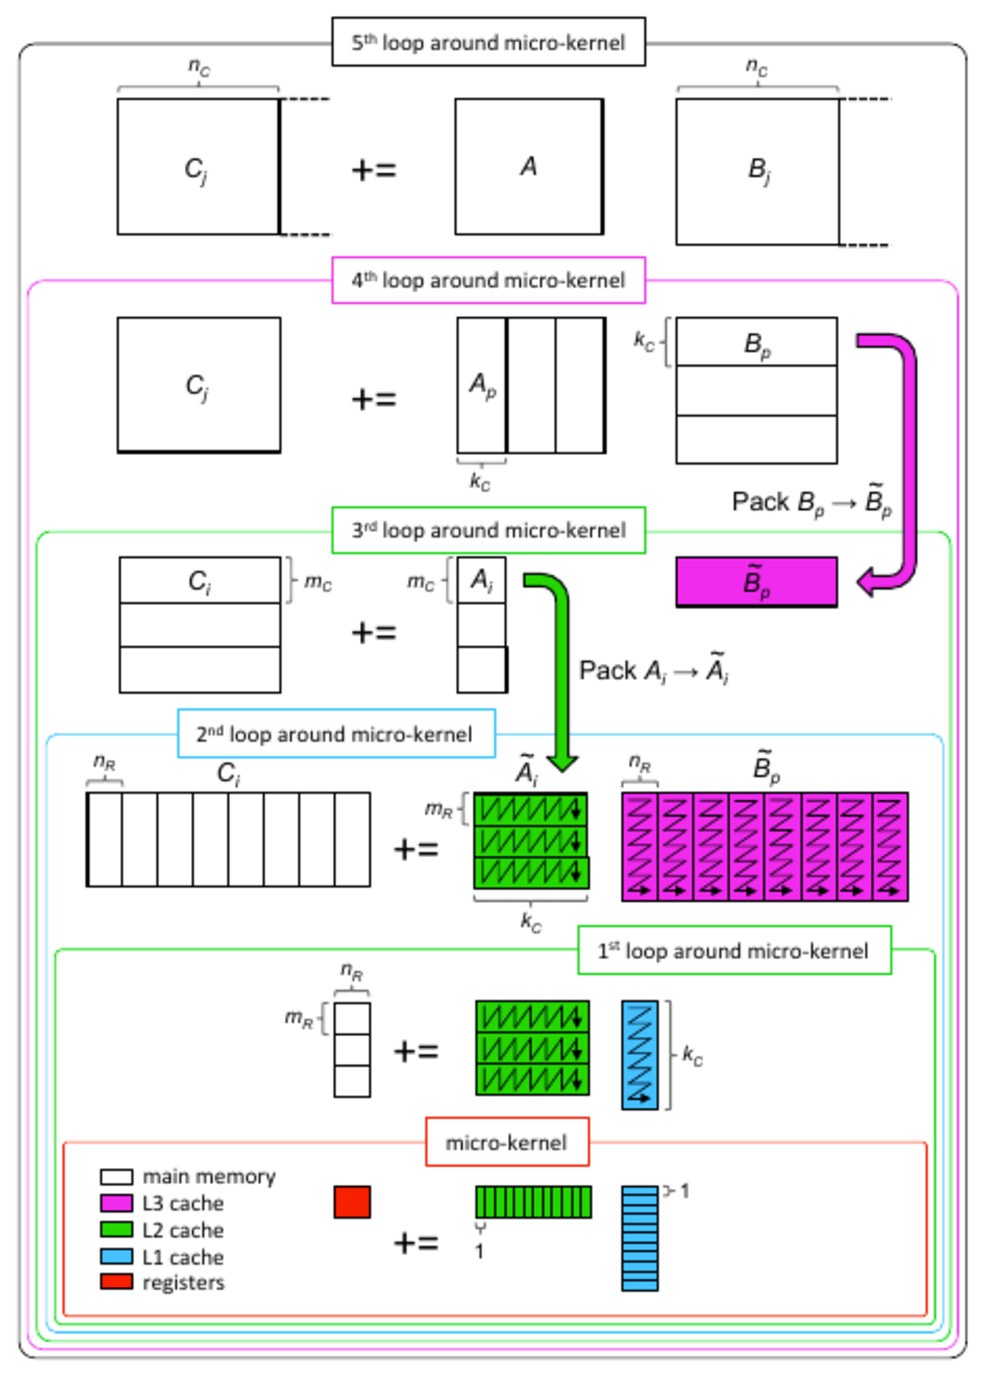
\includegraphics[width=3.0in]{mm_blis_color.pdf}}
		\end{minipage}
		~~~
		\begin{minipage}[t]{3in}
			\footnotesize  
			\mbox{\input blis_gemm_new  }
		\end{minipage}
	\end{center}
	\caption{Left: The GotoBLAS algorithm for matrix-matrix multiplication as  
		refactored in BLIS.  Right: the same algorithm, but expressed as  
		loops.}
	\label{fig:blis_gemm}
\end{figure}

Around 2000, Kazushige Goto revolutionized how \Gemm\ is implemented on current CPUs with his techniques
that were first published in the paper~\cite{Goto:2008:AHP}
\begin{quote}
	Kazushige Goto, Robert A. van de Geijn.
	\myhref{http://dl.acm.org/citation.cfm?id=1356052.1356053&coll=DL&dl=GUIDE&CFID=71223967&CFTOKEN=96440140}{Anatomy of high-performance matrix multiplication.}
	ACM Transactions on Mathematical Software (TOMS).
	Volume 34 Issue 3, May 2008, Article No. 12.
	Also available from 
	 \myhref{http://shpc.ices.utexas.edu/publications.html}{http://shpc.ices.utexas.edu/publications.html}.
\end{quote}
A further ``refactoring'' of this approach was more recently described in~\cite{BLIS1} 
\begin{quote}
	Field G. Van Zee, Robert A. van de Geijn. 
	\myhref{http://dl.acm.org/citation.cfm?id=2786970.2764454&coll=DL&dl=GUIDE&CFID=702354034&CFTOKEN=48470379}{%
		BLIS: A Framework for Rapidly Instantiating BLAS Functionality.} 
	ACM Transactions on Mathematical Software (TOMS).
	Volume 41 Issue 3, June 2015,
	Article No. 14. 
	Also available from \myhref{http://shpc.ices.utexas.edu/publications.html}{http://shpc.ices.utexas.edu/publications.html}.
\end{quote}
The advantage of the BLIS framework is that it reduces the kernel that must be highly optimized, possibly with vector intrinsics or in assemply code, to a {\em micro-kernel}.   In this section, we briefly describe the highlights of the approach.  However, we strongly suggest the reader become familiar with the above two papers themselves.

Figure~\ref{fig:blis_gemm}~(left) illustrates the way the Goto approach structures the blocking for three layers of cache (L1, L2, and L3).  In the BLIS framework, the implementation is structured exactly this way so that only the micro-kernel at the bottom needs to be highly optimized and customized for a given architecture.  In the original GotoBLAS implementation, now maintained as OpenBLAS~\cite{OpenBLASweb}, the operation starting with the second loop around the micro-kernel is instead customized.  In order to get the best performance, it helps is all data is accessed contiguously, which is why at some point prior to reaching the micro-kernel, data is packed in the order indicated by the arrows:
\begin{center}
	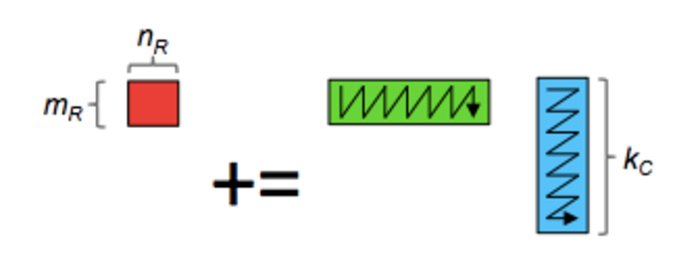
\includegraphics[width=2in]{figures/microkernel.pdf}
\end{center}

Now, notice that each column of the block of $ A $ in the above picture is multiplied by each element in the corresponding row of the block of $ B $.  (We call these blocks of $ A $ and $ B $ {\em micro-panels}.)  This means that the {\em latency} to the L2 cache (the time required to bring in an element of the micro-panel of $ A $ from that cache) can be amortized over $ 2n_R $ flops.  For this reason, we can organize the computation so that the micro-panel of $ A $ typically resides in the L2 cache.  Actually, we can do better: while a rank-1 update is happening with a column of the micro-panels of $ A $ and $ B $, the next column of the micro-panel of $ A $ can be brought into registers so that computation masks the cost of that data movement.
The fact that we want to keep the micro-panel of $ B $ in the L1 cache (because it will be reused for many micro-panels of $ A $) limits the blocking parameter $ k_C $.

With the insights, the rest of the picture hopefully becomes clear.
The first loop around the microkernel works with a block of $ A $, $ \widetilde A_i $, that has been packed and resides in the L2 cache (by virtue of how the computation is ordered).  This limits the blocking parameter $ m_C $.  That block of $ A $ multiplies a block of $ B $, $ \widetilde B_p $, that has been packed to reside in the L3 cache (if the processor has an L3 cache).  Notice that the packing into  $ \widetilde A_i $ is amortized over all computation  with $ \widetilde B_p $ and the packing into $ \widetilde B_p $ is amortized over computations with many blocks $ A_i $.  The outermost loop partitions $ B $ so that the block $ \widetilde B_p $ fits in the L3 cache or, if a processor does not have an L3 cache, limits the amount of workspace for packing $ \widetilde B_p $ that is needed.  This limits the blocking parameter $ n_C $.

One may ask if the above described scheme is optimal.  In~\cite{ITXGEMM:ICCS01} a theory is given that shows that under an idealized model the above is locally optimal (in the sense that assuming data is in a certain memory layer in the hierarchy, the proposed blocking at that level optimally amortizes the cost of data movement with the next memory layer).  A theory that guides the choice of the various blocking parameters is given in~\cite{BLIS4}.

\subsection{Setup}

\begin{figure}[tb!]
	\begin{center}
\begin{minipage}{4in}
	\dirtree{%
		.1 step3.
		.2 README 
%%%\DTcomment{
%%%  \rm \color{red}
%%%  contents of the directory, how to compile and execute the source code{.} 
%%%}
.
		.2 sourceme.sh 
%%%\DTcomment{
%%%			\rm \color{red}
%%%			comment{.} 
%%%		}
.
		.2 makefile 
%%% \DTcomment{
%%%			\rm \color{red}
%%%			comment{.} 
%%%		}
.
		.2 dgemm 
%%%\DTcomment{
%%%			\rm \color{red}
%%%			comment{.} 
%%%		}
.
		.3 my\_dgemm.c 
%%% \DTcomment{
%%%			\rm \color{red}
%%%			comment{.} 
%%%		}
.
		.3 bl\_dgemm\_ref.c 
%%%\DTcomment{
%%%			\rm \color{red}
%%%			comment{.} 
%%%		}
.
		.3 bl\_dgemm\_util.c 
%%% \DTcomment{
%%%			\rm \color{red}
%%%			comment{.} 
%%%		}
.
		.2 include 
%%%\DTcomment{
%%%			\rm \color{red}
%%%			comment{.} 
%%%		}
.
		.3 avx\_types.h 
%%% \DTcomment{
%%%			\rm \color{red}
%%%			comment{.} 
%%%		}
.
		.3 bl\_dgemm.h 
%%% \DTcomment{
%%%			\rm \color{red}
%%%			comment{.} 
%%%		}
.
		.3 bl\_dgemm\_ref.h 
%%%\DTcomment{
%%%			\rm \color{red}
%%%			comment{.} 
%%%		}
.
		.3 bl\_config.h 
%%% \DTcomment{
%%%			\rm \color{red}
%%%			comment{.} 
%%%		}
.
		.3 bl\_dgemm\_kernel.h 
%%% \DTcomment{
%%%			\rm \color{red}
%%%			comment{.} 
%%%		}
.
		.2 kernels
%%%\DTcomment{
%%%			\rm \color{red}
%%%			comment{.} 
%%%		}
.
		.3 bl\_dgemm\_ukr.c
%%%\DTcomment{
%%%			\rm \color{red}
%%%			comment{.} 
%%%		}
%.
%		.3 bl\_dgemm\_int\_8x4.c
%%%%\DTcomment{
%%%%			\rm \color{red}
%%%%			comment{.} 
%%%%		}
%.
%		.3 bl\_dgemm\_asm\_8x4.c
%%%%\DTcomment{
%%%%			\rm \color{red}
%%%%			comment{.} 
%%%%		}
%.
%		.3 bl\_dgemm\_asm\_8x6.c
%%%%\DTcomment{
%%%%			\rm \color{red}
%%%%			comment{.} 
%%%%		}
%.
%		.3 bl\_dgemm\_asm\_12x4.c
%%%%\DTcomment{
%%%%			\rm \color{red}
%%%%			comment{.} 
%%%%		}
.
		.2 lib 
%%%\DTcomment{
%%%			\rm \color{red}
%%%			comment{.} 
%%%		}
.
        .3 libblislab.a
%%% \DTcomment{
%%%			\rm \color{red}
%%%			comment{.} 
%%%		}
.
        .3 libblislab.so
%%% \DTcomment{
%%%			\rm \color{red}
%%%			comment{.} 
%%%		}
.
		.2 make.inc.files
%%% \DTcomment{
%%%			\rm \color{red}
%%%			comment{.} 
%%%		}
.
		.3 make.intel.inc 
%%% \DTcomment{
%%%			\rm \color{red}
%%%			comment{.} 
%%%		}
.
		.3 make.gnu.inc 
%%%\DTcomment{
%%%			\rm \color{red}
%%%			comment{.} 
%%%		}
.
		.3 make.inc 
%%% \DTcomment{
%%%			\rm \color{red}
%%%			comment{.} 
%%%		}
.
		.2 test 
%%%\DTcomment{
%%%			\rm \color{red}
%%%			comment{.} 
%%%		}
.
		.3 makefile 
%%% \DTcomment{
%%%			\rm \color{red}
%%%			comment{.} 
%%%		}
.
		.3 test\_bl\_dgemm.c 
%%%\DTcomment{
%%%			\rm \color{red}
%%%			comment{.} 
%%%		}
.
		.3 run\_bl\_dgemm.sh 
%%% \DTcomment{
%%%			\rm \color{red}
%%%			comment{.} 
%%%		}
.
		.3 test\_bl\_dgemm.x 
%%%\DTcomment{
%%%			\rm \color{red}
%%%			comment{.} 
%%%		}
.       
		.3 tacc\_run\_bl\_dgemm.sh 
%%% \DTcomment{
%%%			\rm \color{red}
%%%			comment{.} 
%%%		}
.	
	}
\end{minipage}
\end{center}
\caption{Structure of directory {\tt step3}.}
\label{fig:DirStep1}
\end{figure}

Figure~\ref{fig:DirStep1} illustrates the directory
structure for subdirectory {\tt step3}. Comparing to {\tt step1}, we have modified/added the following directories/files:

\begin{description}
\item[{\tt kernels}] This directory contains the micro-kernel implementations for various architecture.
\begin{description}
\item[{\tt bl\_dgemm\_ukr.c}] gives a naive C implementation.
%\item[{\tt bl\_dgemm\_int\_8x4.c}] Is an {\tt AVX} intrinsics micro-kernel implementation for Sandy Bridge/Ivy Bridge micro-architecture.
%\item[{\tt bl\_dgemm\_asm\_8x4.c}] Is an {\tt AVX} assembly micro-kernel implementation for Sandy Bridge/Ivy Bridge micro-architecture.
%\item[{\tt bl\_dgemm\_asm\_8x6.c}] Is an {\tt AVX2} assembly micro-kernel implementation for Haswell micro-architecture.
%\item[{\tt bl\_dgemm\_asm\_12x4.c}] Is an alternative {\tt AVX2} assembly micro-kernel implementation for Haswell micro-architecture.
\item[{\tt bl\_dgemm\_int\_kernel.c}] gives an {\tt AVX/AVX2} intrinsics micro-kernel implementation for Haswell architecture.
\item[{\tt bl\_dgemm\_asm\_kernel.c}] gives an {\tt AVX/AVX2} assembly micro-kernel implementation for Haswell architecture.
\end{description}
\end{description}

\subsection{Advanced techniques}
%{\bf Describe vector instructions and how to access them through vector intrinsics.}
You can find the vector instructions online:
\begin{itemize}
\item \myhref{https://software.intel.com/sites/landingpage/IntrinsicsGuide/}{Intel Intrinsics Guide}
\item \myhref{https://software.intel.com/en-us/isa-extensions}{Intel ISA Extensions}
\end{itemize}

\subsubsection{An introduction example for ``{\tt axpy}''}
We provide you an example for the implementation of ``{\tt axpy}'' to demostrate how to use Intel {\tt AVX} Intrinsics and Assembly (in {\tt src/examples} subdirectory). This example will serve as a good start point for you to learn basic {\tt broacast}/{\tt fma}/{\tt load}/{\tt store} instructions. Moreover, this example is actually a primitive for the ``broadcast'' implementation for 4$\times$4 rank-1 update.

\subsubsection{4$\times$4 rank-1 update}
The micro-kernel implementation can be boiled down to a 4$\times$4 rank-1 update. There are two possible implementation: one based on broadcast (Figure~\ref{fig:broadcast}) and and one of a butterfly permutation (Figure~\ref{fig:permutation}). You can also try other possible implementations.
\begin{figure}
\begin{center}
	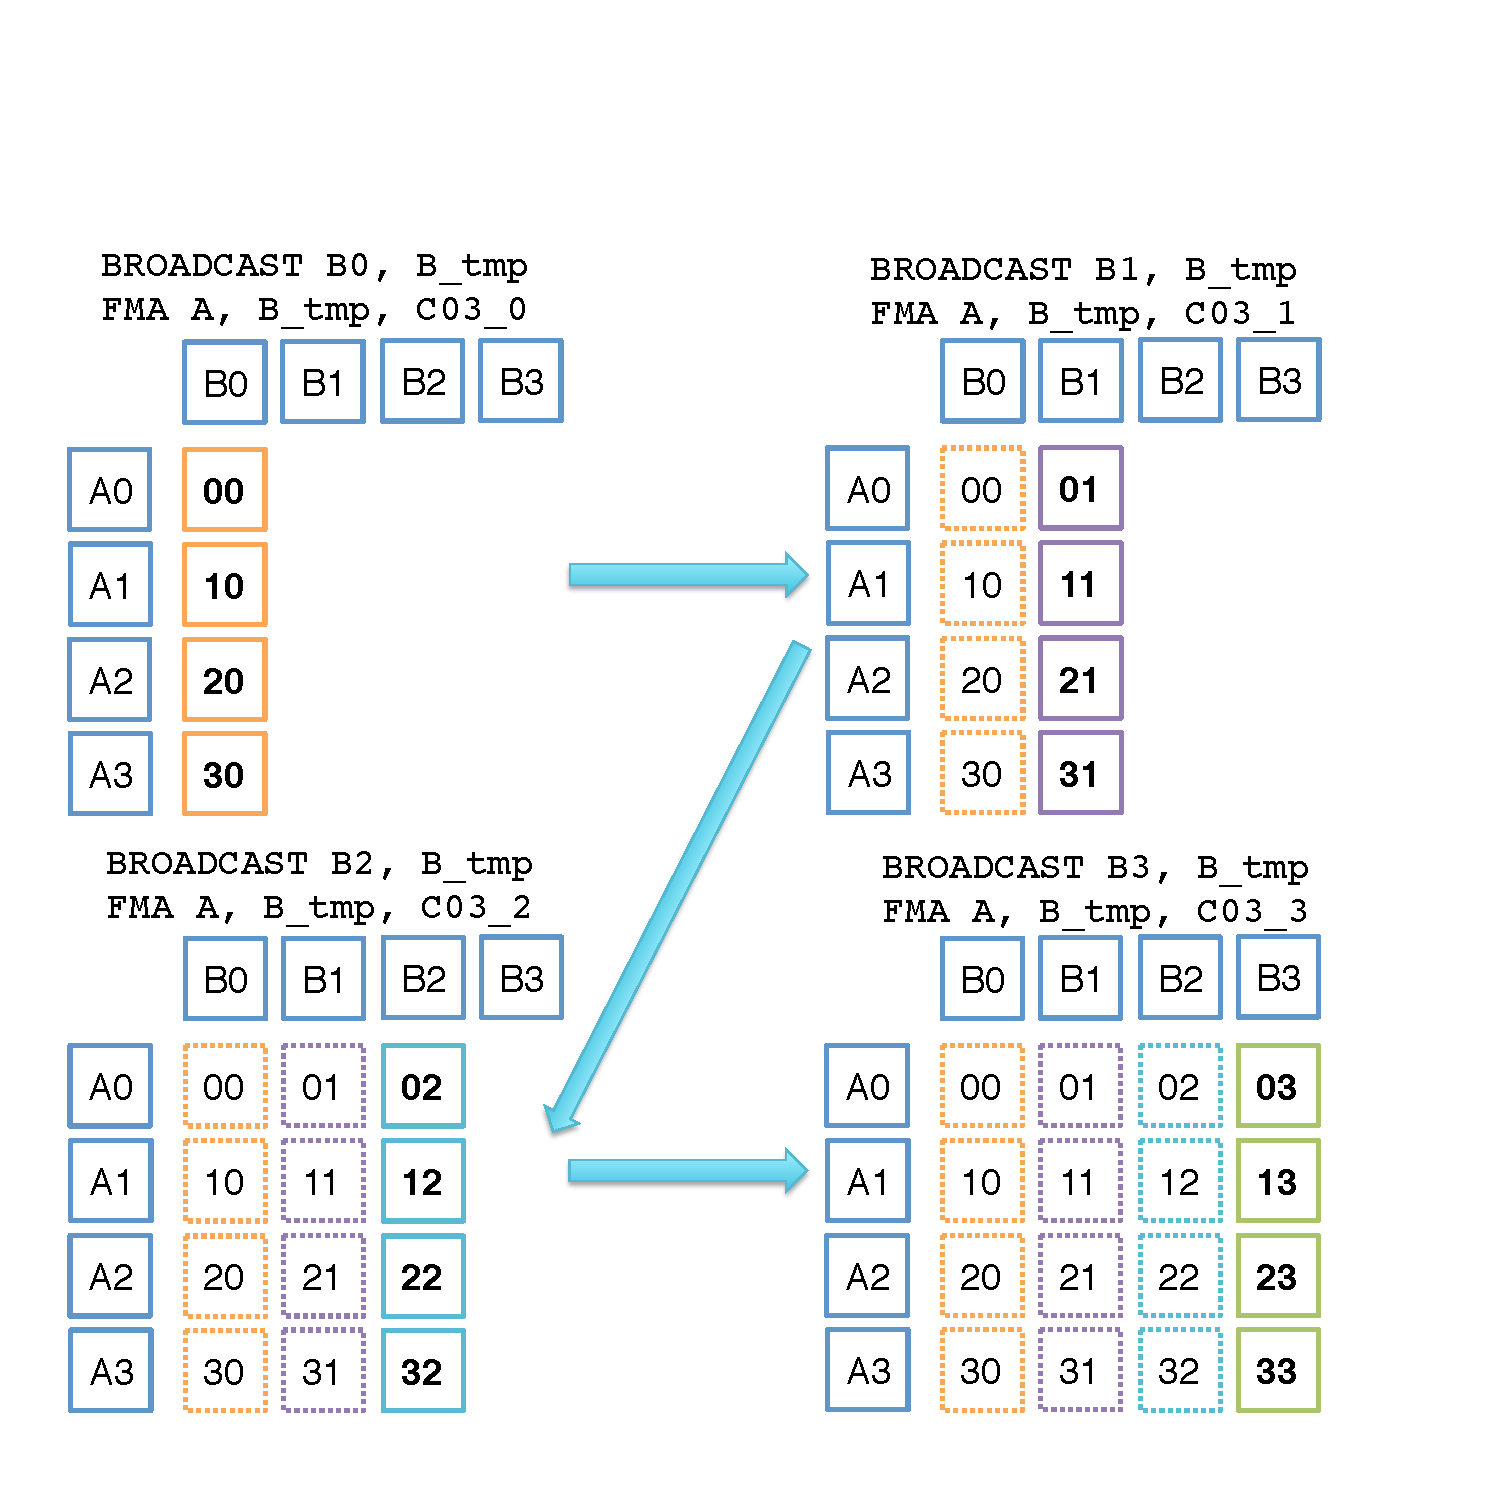
\includegraphics[width=5in]{figures/avx_broadcast.pdf}
\end{center}
\caption{{\tt AVX} 4$\times$4 rank-1 update with broadcast. Given 4$\times$1 vector $A$ and $B$, we compute the 4$\times$4 outer-product C by 4 {\tt FMA} interleaved with vectorized broadcast operations.}
\label{fig:broadcast}
\end{figure}

\begin{figure}
\begin{center}
	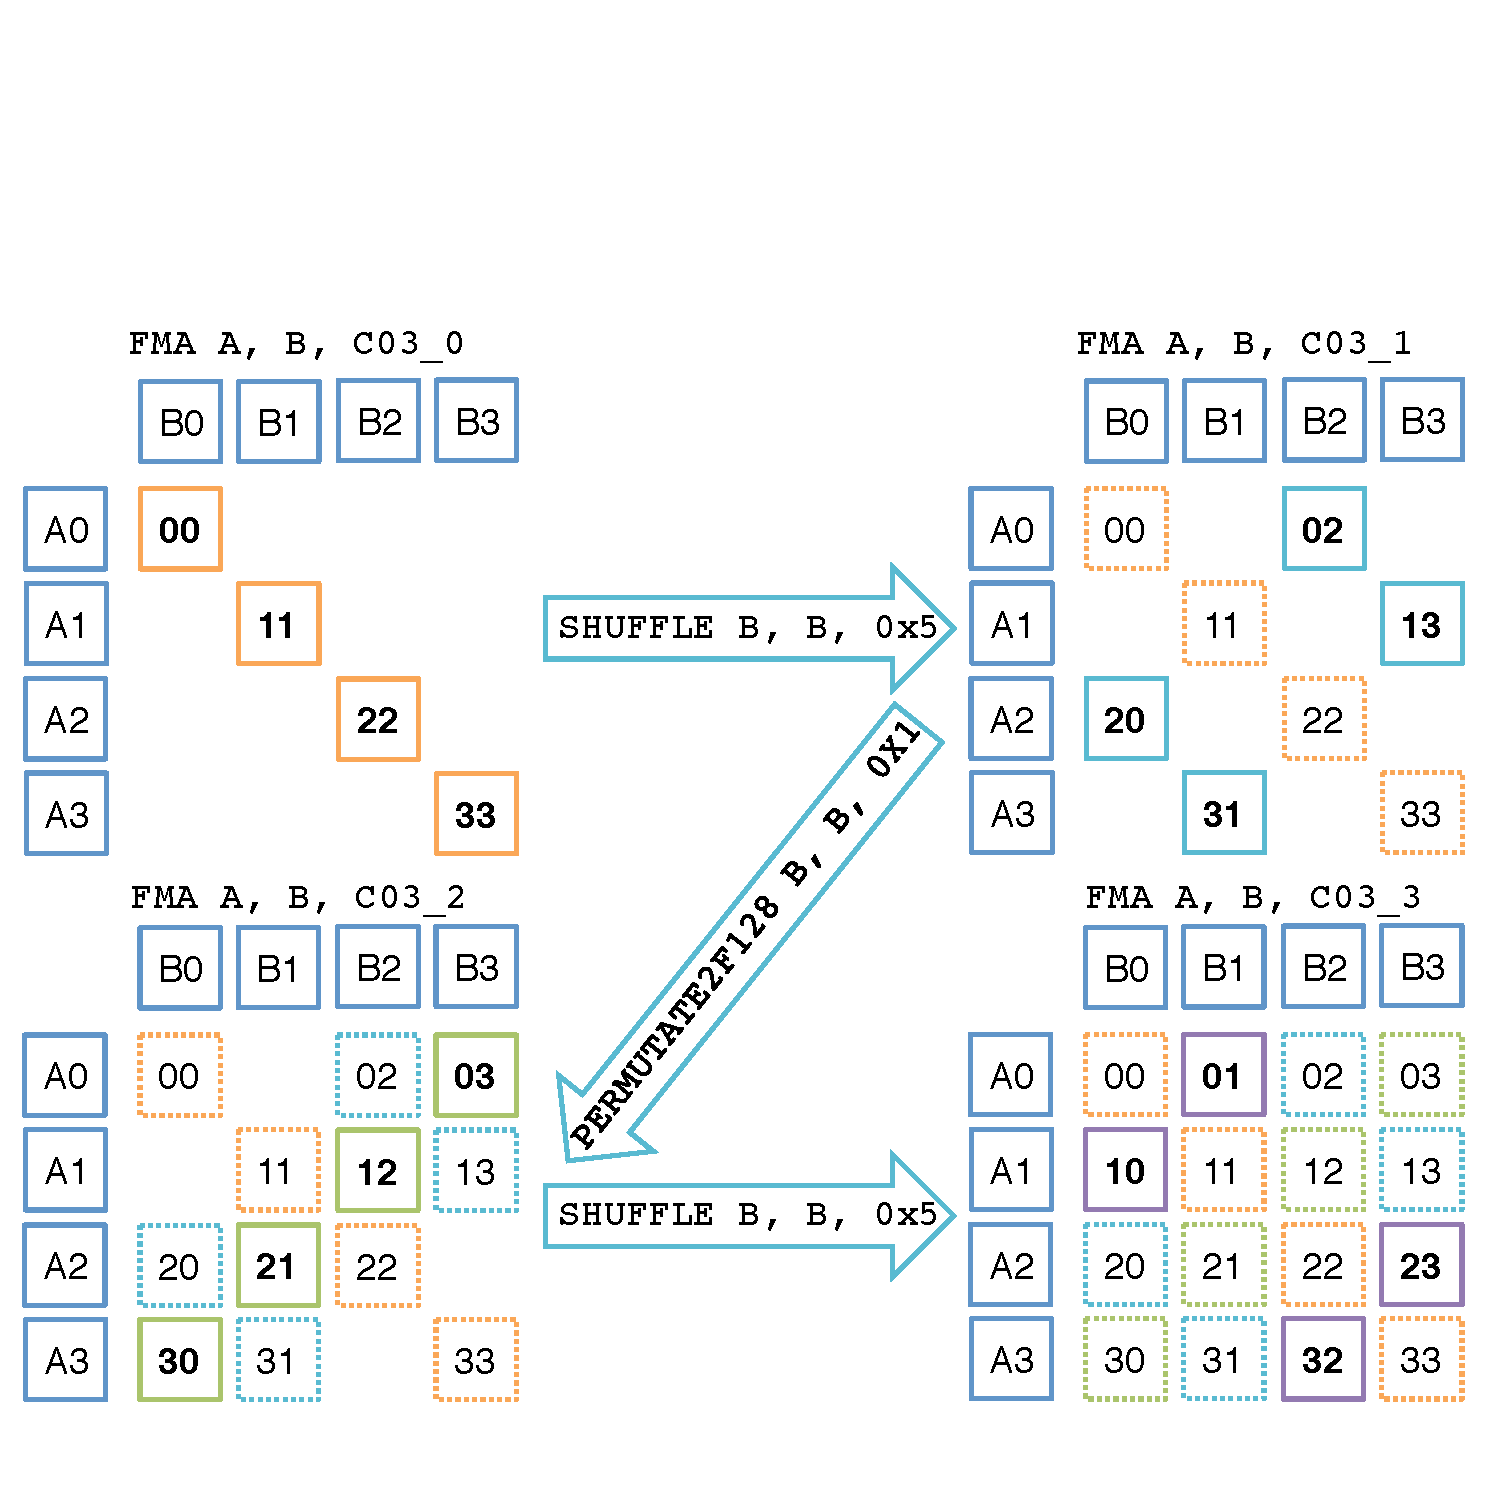
\includegraphics[width=5in]{figures/avx_permute.pdf}
\end{center}
\caption{{\tt AVX} 4$\times$4 rank-1 update with butterfly permutation. Given 4$\times$1 vector $A$ and $B$, we compute the 4$\times$4 outer-product C by 4 {\tt FMA} interleaved with vectorized shuffling operations. The 3rd operands (0x5, 0x1) indicates the shuffling (permutation) type.}
\label{fig:permutation}
\end{figure}

\subsection{Your mission, if you choose to accept it}
We provide you a reference implementation of simplified BLIS framework in {\tt my\_dgemm}. The code is organized in the same way presented in Figure~\ref{fig:blis_gemm}. However, the step size in each loop is not well choosen, and the micro-kernel implementation is a naive {\tt C} version. Therefore. you will not expect high performance with the code. What we want you to do is to 
\begin{itemize}
\item Specify the blocking parameter $ m_C $, $ n_C $, $ k_C $ and the micro-kernel size parameter $ m_R $, $ n_R $ in the file {\tt include/bl\_config.h}; and
\item Implement the efficient micro-kernel with vector intrinsics or assembly code. Place the code in {\tt kernels/bl\_dgemm\_int\_kernel.c} (for vector intrinsics), or {\tt kernels/bl\_dgemm\_asm\_kernel.c} (for assembly). You need to specify the function name of the micro-kernel by modifying {\tt BL\_MICRO\_KERNEL} in {\tt include/bl\_config.h}.
\end{itemize}

